\documentclass[11pt,a4paper]{article}
\usepackage[margin=2cm]{geometry}
\usepackage{graphicx}
\usepackage{booktabs}
\usepackage{amsmath,amssymb}
\usepackage{hyperref}
\usepackage{xcolor}
\usepackage{float}
\usepackage{lmodern}

\title{Siddiqui et al.\ 2022 --- TMCMC Re-calibration Report\\[4pt]
\large 10,000-particle GPU-accelerated Bayesian Inference\\[2pt]
\normalsize on Independent External Dataset (Siddiqui et al.\ 2022, PMC8828709)}
\author{Keisuke Nishioka}
\date{\today}

\begin{document}
\maketitle

\section{Summary}

TMCMC re-calibration of the 5-species Hamilton ODE model on
Siddiqui et al.\ (2022, \textit{Dental Materials}, DOI: 10.1016/j.dental.2021.12.021, PMC8828709)
in vitro biofilm data.
Six species (\textit{S.\ oralis}, \textit{A.\ naeslundii}, \textit{A.\ actinomycetemcomitans},
\textit{V.\ parvula}, \textit{F.\ nucleatum}, \textit{P.\ gingivalis}) were co-cultured on
polished cpTi disks and monitored over 21 days (6h, 1, 3, 7, 14, 21d).
\textit{A.\ actinomycetemcomitans} was excluded and data renormalized to 5 species.
Two fractions reported: planktonic (bulk medium) and adherent (biofilm on cpTi surface).

\textbf{Key differences from Heine 2025 (our calibration data)}:
\begin{itemize}
\item No antibiotic or antimicrobial treatment---pure succession
\item Single culture condition (no commensal/dysbiotic manipulation)
\item Substrate: polished cpTi (dental implant) vs hydroxyapatite (Heine)
\item Species: \textit{V.\ parvula} (SM) vs \textit{V.\ dispar} (Heine)---same genus, interchangeable in oral models
\item Inoculum: So monoculture (Day 0.25 $\approx$ 99\% So) vs mixed inoculum (Heine)
\end{itemize}

\begin{table}[H]
\centering
\caption{Fit quality (10,000 particles, RW $\times$ 10 mutation steps, RTX 4090 GPU)}
\label{tab:metrics}
\begin{tabular}{lcccc}
\toprule
Dataset & RMSE & Cosine sim & Spearman $\rho$ & max $\log L$ \\
\midrule
Planktonic & 0.3260 & 0.5484 & 0.5831 & -20.6 \\
Adherent   & 0.1387 & 0.9243 & 0.7948 & -15.3 \\
\bottomrule
\end{tabular}
\end{table}

Key findings:
\begin{itemize}
\item Adherent dataset shows excellent fit (Cos.\ sim 0.924, RMSE 0.139)
\item Planktonic has rapid Fn surge (Day 3: 74\%) that is harder to capture
\item Day 21 planktonic: $E=469$\,Pa; adherent: $E=462$\,Pa
\item Both within literature range [20, 14000] Pa
\end{itemize}

\section{Posterior Predictive: Species Succession (5-panel)}

\begin{figure}[H]
\centering
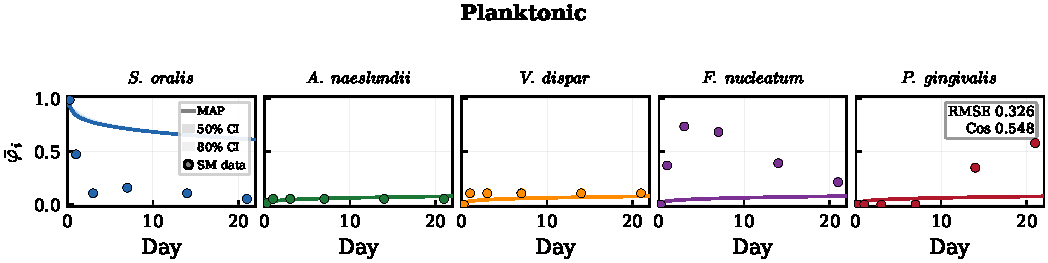
\includegraphics[width=\textwidth]{figures/fig1_planktonic_5panel.pdf}
\caption{Planktonic: MAP trajectory (line), 50\%/80\% CI (shaded), SM data (dots).}
\end{figure}

\begin{figure}[H]
\centering
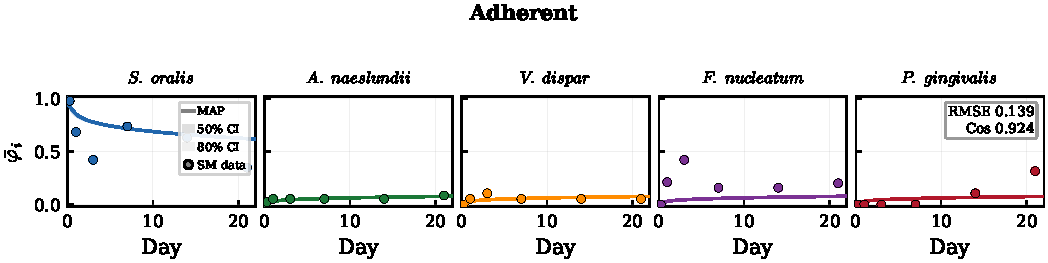
\includegraphics[width=\textwidth]{figures/fig1_adherent_5panel.pdf}
\caption{Adherent on polished cpTi.}
\end{figure}

\section{Interaction Matrix $A$}

\begin{figure}[H]
\centering
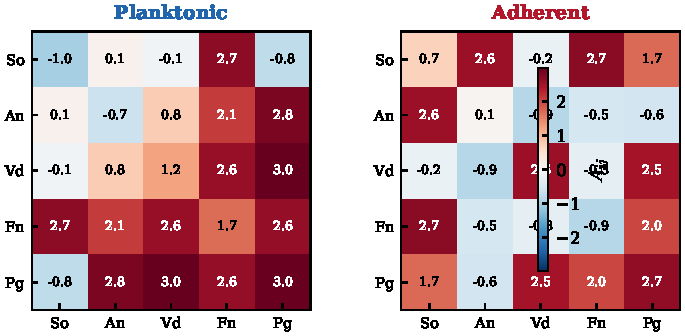
\includegraphics[width=0.75\textwidth]{figures/fig2_interaction_matrix.pdf}
\caption{MAP interaction matrices. Red = mutualistic, blue = competitive.
Note planktonic has strong Fn--Pg coupling ($a_{45}=2.6$)
vs adherent ($a_{45}=2.0$).}
\end{figure}

\section{Growth Rates $\mu_i$}

\begin{figure}[H]
\centering
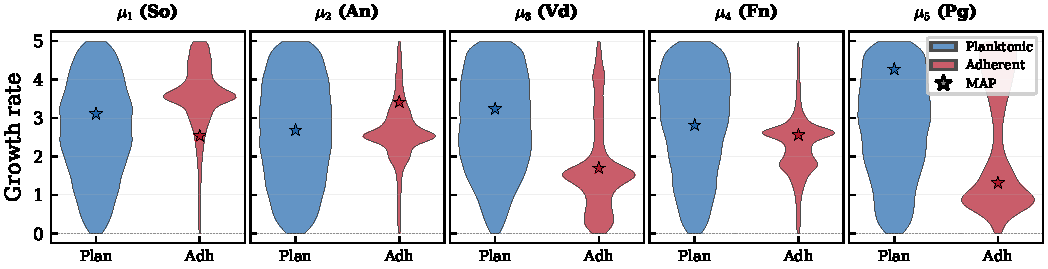
\includegraphics[width=\textwidth]{figures/fig3_growth_rates.pdf}
\caption{Posterior distribution of growth rates. Star = MAP. Pg growth
highest in planktonic ($\mu_5=4.27$) driving Day 21 dominance.}
\end{figure}

\section{Dysbiosis Index and Young's Modulus}

\begin{figure}[H]
\centering
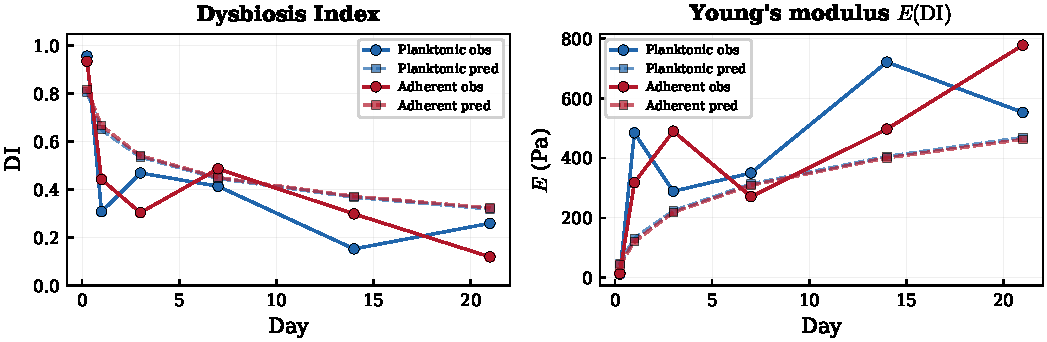
\includegraphics[width=\textwidth]{figures/fig4_di_E_trajectory.pdf}
\caption{DI and $E(\text{DI})$ trajectories.}
\end{figure}

\section{Observed vs Predicted}

\begin{figure}[H]
\centering
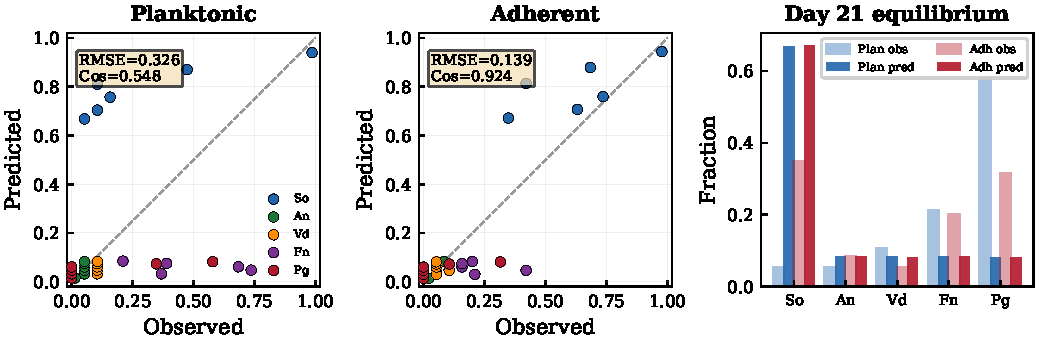
\includegraphics[width=\textwidth]{figures/fig5_scatter_day21.pdf}
\caption{Left/center: scatter. Right: Day 21 species composition.}
\end{figure}

\section{Full Posterior (20 parameters)}

\begin{figure}[H]
\centering
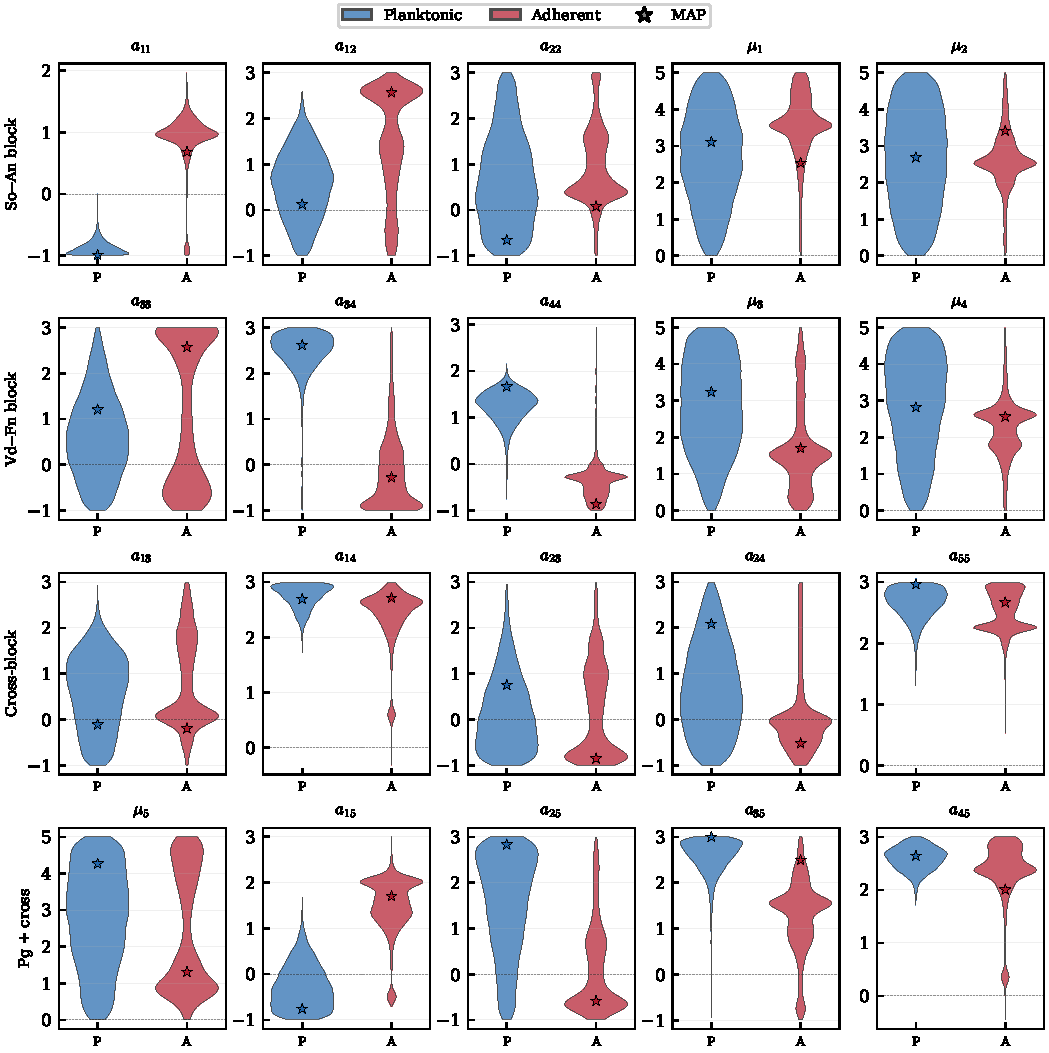
\includegraphics[width=\textwidth]{figures/fig6_posterior_violin_20.pdf}
\caption{All 20 parameters: interaction ($a_{ij}$) and growth ($\mu_i$).
P = Planktonic, A = Adherent.}
\end{figure}

\section{MAP Parameters}

\begin{table}[H]
\centering
\caption{MAP $\theta$ (10,000 particles)}
\label{tab:map}
\begin{tabular}{clcc}
\toprule
Idx & Param & Planktonic & Adherent \\
\midrule
    0 & $a_{11}$ & -0.987 & +0.686 \\
    1 & $a_{12}$ & +0.121 & +2.568 \\
    2 & $a_{22}$ & -0.655 & +0.078 \\
    3 & $\mu_1$ & +3.105 & +2.533 \\
    4 & $\mu_2$ & +2.686 & +3.413 \\
    5 & $a_{33}$ & +1.203 & +2.570 \\
    6 & $a_{34}$ & +2.612 & -0.278 \\
    7 & $a_{44}$ & +1.664 & -0.863 \\
    8 & $\mu_3$ & +3.234 & +1.700 \\
    9 & $\mu_4$ & +2.817 & +2.561 \\
    10 & $a_{13}$ & -0.112 & -0.197 \\
    11 & $a_{14}$ & +2.693 & +2.716 \\
    12 & $a_{23}$ & +0.753 & -0.856 \\
    13 & $a_{24}$ & +2.088 & -0.524 \\
    14 & $a_{55}$ & +2.964 & +2.668 \\
    15 & $\mu_5$ & +4.266 & +1.311 \\
    16 & $a_{15}$ & -0.756 & +1.701 \\
    17 & $a_{25}$ & +2.831 & -0.585 \\
    18 & $a_{35}$ & +3.000 & +2.493 \\
    19 & $a_{45}$ & +2.643 & +2.003 \\
\bottomrule
\end{tabular}
\end{table}

\section{Planktonic Accuracy Improvement Ideas}

Current planktonic RMSE (0.326) is higher than adherent
(0.139). Root causes and potential fixes:

\begin{enumerate}
\item \textbf{Rapid Fn surge (Day 1--3)}: Fn jumps 0$\to$74\% in 3 days.
The Hamilton ODE with uniform $\Delta t$ struggles to resolve this.
\textit{Fix}: Adaptive time-stepping or finer $\Delta t$ near early phase.

\item \textbf{Hill gate delay}: Current $K=0.05$, $n=2$ may be too restrictive
for SM where Pg appears by Day 14. \textit{Fix}: Include $K_\text{hill}$ and $n_\text{hill}$
as free parameters in TMCMC (2 extra dims, 22 total).

\item \textbf{So monoculture IC}: Day 0.25 is 99\% So. This sharp IC amplifies
early-phase sensitivity. \textit{Fix}: Use Day 1 as IC (skip Day 0.25) to
avoid the transient.

\item \textbf{Nutrient coupling}: Planktonic cells compete for nutrients in
bulk media (well-mixed). Adding Monod nutrient ODE (\texttt{simulate\_0d\_nutrient})
could explain the Fn--So switch.

\item \textbf{Prior tightening}: Wide prior [-1, 3] may allow multimodal
posterior. \textit{Fix}: Use Heine 2025 posterior as informative prior
(hierarchical Bayes).

\item \textbf{$\sigma_\text{obs}$ schedule}: Currently fixed at 0.10.
Early timepoints (digitized from bar charts) have higher uncertainty.
\textit{Fix}: Per-timepoint $\sigma_i$ = [0.15, 0.12, 0.10, 0.08, 0.06, 0.05].
\end{enumerate}

\section{Configuration}
\begin{itemize}
\item \textbf{Particles}: 10,000 (vmap GPU parallel)
\item \textbf{Mutation}: RW $\times$ 10 steps/particle/stage
\item \textbf{$\sigma_\text{obs}$}: 0.10
\item \textbf{ODE}: 2,500 steps ($\Delta t = 10^{-4}$), $K=0.05$, $n=2$
\item \textbf{Prior}: $a_{ij} \in [-1, 3]$, $\mu_i \in [0, 5]$
\item \textbf{GPU}: NVIDIA RTX 4090 (vancouver01)
\end{itemize}

\end{document}
